\documentclass[12pt]{article}
\usepackage[top=1.5cm, bottom=1.25cm, left=2cm, right=2cm]{geometry}

\usepackage[spanish,activeacute]{babel}
\usepackage{amssymb,amsmath}
\usepackage{enumerate}
\usepackage{verbatim}
\usepackage{array}
\usepackage{hyperref}
\usepackage{graphicx}
\usepackage{url}
\usepackage{fontspec}

\setmainfont{Roboto Condensed}
%\renewcommand{\familydefault}{\sfdefault}

\begin{document}



\pagestyle{plain}


\setlength{\unitlength}{1cm}
%
%\setlength{\extrarowheight}{5mm}
%

\begin{flushright}
{\setmainfont{STIX}\small\textit{
``40 años de la Convención sobre la eliminación de Todas las Formas de Discriminación contra la Mujer''}
}
\end{flushright}


\noindent\begin{tabular}{m{.1\textwidth} }
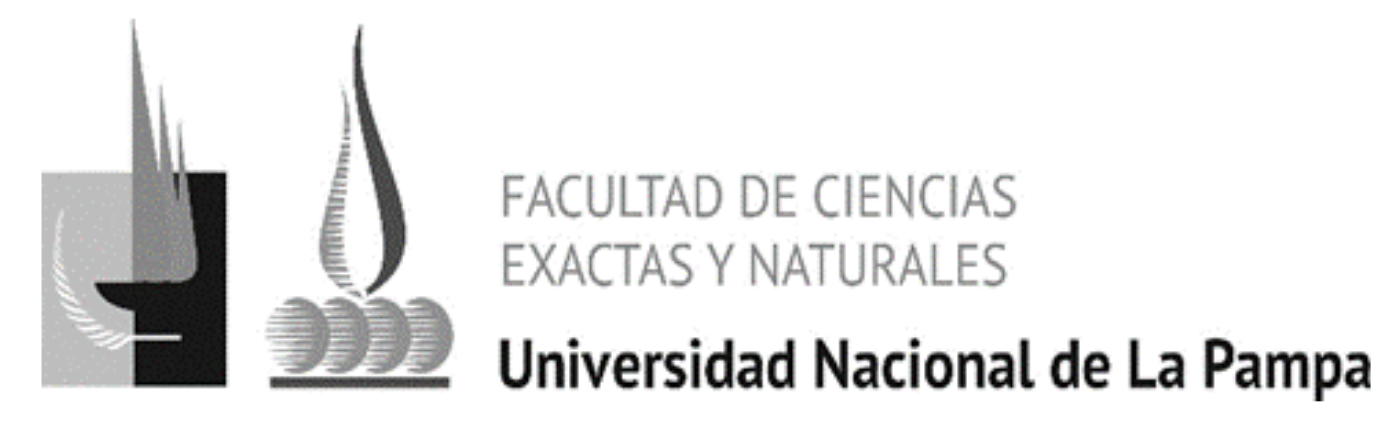
\includegraphics[scale=.25]{EscudoUNLPam.png} 

%\end{large}
\\
\end{tabular}

\setlength{\parindent}{0pt} % Default is 15pt.

\begin{center}
 \textbf{\Large Programa Actividades Curriculares}
\end{center}





 \textbf{Departamento:}  Matemática.

 \textbf{Actividad Curricular:} Topología II

 \textbf{Carrera y Plan:}  Lic. en Matemática Plan de Estudios RCS 008/90.

\textbf{Curso:} Tercer Año

\textbf{Regimen:} Cuatrimestral

\textbf{Carga Horaria Semanal:} Teóricos 4hs, Prácticos 6hs. 

\textbf{Carga Horaria Total:} Teóricos 40hs, Prácticos 60hs.

\textbf{Ciclo Lectivo:} 2019



\textbf{Equipo Docente:}  

\begin{table}[h]
\begin{tabular}{|l|l|l|l|l|}\hline
& Nombre & Cargo  & Dedicación & Caracter\\ \hline
Teórico & Fernando Mazzone & Prof. Titular & Simple & Regular\\\hline
Práctico & Sonia Acinas & Prof. Adjunto & Exclusiva & Regular\\\hline 
\end{tabular} 
\end{table}

\textbf{Fundamentación.}

\begin{itemize}
 \item \textbf{Importancia Matemática de los Contenidos Seleccionados.}  La introducción en la problemática de la convergencia de funciones y en la teoría de la medida e integración forma parte de la curricula obligatoria de casi todas las carreras de Lic. en Matemática del país. La integral de Lebesgue es una pieza clave donde se asientan  muchas otras contrucciones del saber matemático, por ejemplo los espacios de funciones que son de una importancia clave a la hora de mostrar que problemas  relacionados con ecuaciones diferenciales tienen solución. La integral de Lebesgue nos proporciona  un instrumento preciso para manipular determinadas expresiones, principalmente por su capacidad de interactuar con otro  concepto central del análisis. Nos referimos al concepto \emph{límite} en sus múltiples manifestaciones: sucesiones, series, derivadas, etc. El concepto de medida mostro además ser fecundo a la hora de introducir nuevos conceptos como derivadas débiles, soluciones débiles y distribuciones. 

\item \textbf{Contextualización del estudiante.} Los contenidos han sido elegidos de modo de atender las características en cuanto a la formación que presentan los estudiantes. Por este motivo se  incluyen y desarrollan conceptos como, convergencia de series numéricas y criterios de convergencia, cardinalidad, Teorema de Heine-Borel y funciones uniformemente continuas, Integral de Riemann, entre otros. Estos temas muchas veces a pesar de haber sido estudiados por el alumno los tiene olvidados al momento de la cursada, especialmente porque suele ser el caso que curso las asignatura donde fue introducido a ellos  varios años antes.


\item \textbf{Uso de herramientas computacionales.}  En nuestra opinión  la capacidad para utilizar  herramientas computacionales de cálculo numérico y simbólico para plantear y resolver problemas es una competencia imprescidible en un estudiante de Lic. en Matemática. Las mencionadas herramientas permiten realizar cálculos numéricos y de manipular expresiones  que  por sus dimensiones sería imposible desarrollar  de otra forma que no sea asistido por una computadora. Además que la habilidad en la utilización de instrumentos informáticos repercute en mejorar la calificación laboral del futuro egresado. Así pensamos que se debe recurrir de manera intensiva  a estos rescursos, no sólo en los expacios curriculares destinados específicamente a ellos sino en otros Topología II. Nuestro plan es hacer una  introducción sumaria  al alumno al lenguaje de programación Python y a la librería de cálculo simbólico de este lenguaje SymPy y usar ella para realizar gráficos y como instrumento empírico para chequear determinadas relaciones.

\item \textbf{Enfoque metodológico en la enseñanza.} Una de las principales dificultades en la enseñanza  de la medida e integral de Lebesgue se puede apreciar cuando se toma dimensión histórica de este concepto.  Este instrumento matemático fue elaborado por sucesivas aproximaciones en el lapso de los dos milenios que median entre el método de exhausción de los antiguos griegos y las obras de Henri Lebesgue Leçons sur l'intégration et la recherché des fonctions primitives (1904) y Leçons sur les séries trigonométriques (1906). Tiene origen en varias problemáticas que preocupan a los matemáticos, particularmente  la convergencia de las series de Fourier y la caracterización de la funciones integrables Riemann. 

Somos de la opinión que un elemento importante para prestar atención en el proceso de enseñanza-aprendizaje es la cuestión del sentido. El alumno debe percibir que el concepto que se le pretende enseñar tiene un sentido y razón de ser. En ese sentido nos parece importante que además de exponer los aspectos lógicos y formales que fundamentan la nociones de esta materia debemos preocuparnos por aquellos elementos que motivan su existencia. 

Adherimos a I. Kleiner en \emph{Excursions in the History of Mathematics}, cuando dice:

\begin{quote}
<<La enseñanza del cálculo, qué debe enseñarse y cómo debe enseñarse, es
un tema bajo debate continuo...

Como señalamos anteriormente, el cálculo involucra algoritmos, teoría y aplicaciones.
En cierto punto, entonces, los estudiantes deben estar expuestos a su poder técnico, su 
armonía lógica  y su utilidad. El cálculo es también la respuesta a una búsqueda de 2000 años para describir la continuidad y la variabilidad; es un logro intelectual enorme. El espíritu de estos pensamientos debe animar nuestra enseñanza del tema, las ideas centrales deben destacar entre los cientos de fórmulas y técnicas.

Hilbert observó que cada teoría matemática pasa por tres períodos de
desarrollo: lo ingenuo, lo formal y lo crítico. En el caso del cálculo, el
período ingenuo ocurrió en el siglo XVII, el formal en el siglo XVIII, y
la crítica en el XIX. La evolución de una idea matemática a menudo procede.
en cuatro etapas: descubrimiento (o invención), uso, comprensión y justificación . Es importante mantener el orden de estas etapas en mente al discutir cualquier concepto o teoría.>>
\end{quote}

La temática de la enseñanza del análisis matemático tomado en consideración  la evolución histórica del mismo ha recido atención en la bibliografía reciente, en especial de habla inglesa, por ejemplo en \cite{bressoud2008radical,hawkins2001lebesgue, bressoud2007radical,abbott2002understanding,hairer2008analysis}.


\end{itemize}

\textbf{Objetivos}
\begin{itemize}
 \item Introducir al alumno al problema de convergencia de: sucesiones, series, productos infinitos, series de potencias y series de Fourier.
 \item Hacer un examen crítico de la integral de Riemann, precisar sus alcances y límites
 \item Introducir al alumnos a las nociones de medida e integral de Lebesgue. 
 \item Percibir la potencia instrumental de la integral de Lebesgue por sobre la integral de Riemann.
 \item Desarrollar el pensamiento analítico tendiente a justificar con rigor matemático todas las distintas afirmaciones.
 \item Utilizar herramienta de cálculo como medio de mecanismo empírico de conocimiento.
 \item Desarrollar la capacidad de resolver problemas.
 \item Incentivar el espíritu crítico, entiendiendo por esto la capacidad  de analizar un razonamiento formal, de preguntarse por la razón de ser de una teoría y de interpelarnos sobre creencias arraigadas en nuestro pensamiento. 
\end{itemize}

\newpage








\begin{center}
 {\Large \bfseries Programa analítico} 
\end{center}




\begin{description}
 \item[Unidad 0. Python y SymPy.] Panorama de instalación, distribuciones y recursos online. Tipos de datos en Python, programación elemental.

\item[Unidad 1. Preliminares] Cardinalidad. Conjuntos numerables. Potencia del continuo. Topología en los espacios Euclideos $\mathbb{R}^n$. Completitud. Supremo e ínfimo. Compacidad, Teoremas de Bolzano-Weiertrass y Heine-Borel. Funciones uniformemente continuas. Sucesiones numéricas. Convergencia de sucesiones monótonas. El límite inferior y el límite superior. Series numéricas, productos infinitos. Criterios de convergencia. 


\item[Unidad 3. Convergencia de funciones] Sucesiones de funciones. Convergencia puntual. La convergencia puntual y: la continuidad, la derivada y la integral. Convergencia uniforme. Series de funciones y productos infinitos. El criterio $M$-test de Weiertrass. Convergencia de series de potencias. Series de Fourier. Coeficientes de Fourier. Polinomios de Berstein. Teorema de aproximación de Weiertrass.

\item[Unidad 2. La integral de Riemann] Sumas superiores e inferiores de de Darboux. Funciones Integrables Riemann. Ejemplos de función no integrable Riemann. Diversos ejemplos de funciones integrables Riemann discontinuas sobre conjuntos densos.  Criterio de integrabilidad de Riemann. Contenido exterior de conjuntos. Criterio de intregrabilidad de Hankel. 

\end{description}













%
%
\nocite{*}
\bibliographystyle{apalike-url}
  \bibliography{biblio}

\end{document}
